\documentclass[conference]{IEEEtran}
\IEEEoverridecommandlockouts

\usepackage{cite}
\usepackage{amsmath,amssymb,amsfonts}
\usepackage{graphicx}
\usepackage{textcomp}
\usepackage{xcolor}
\usepackage{float}
\usepackage{hyperref}
\usepackage{listings}

\def\BibTeX{{\rm B\kern-.05em{\sc i\kern-.025em b}\kern-.08em
    T\kern-.1667em\lower.7ex\hbox{E}\kern-.125emX}}
\begin{document} 


\title{Activity 8: Noise Analysis}

\author{\IEEEauthorblockN{Emmanuel Jesus R. Estallo}
\IEEEauthorblockA{\textit{Electrical and Electronics Engineering Institute} \\
\textit{University of the Philippines - Diliman}\\
Quezon City, Philippines\\
emmanuel.estallo@eee.upd.edu.ph}}

\maketitle
\section{Transistor Noise}
\subsection{NMOS Noise}
For the NMOS with VDS = VGS = 900mV, $I_D=439\mu A$. Additionally, $g_m=2.44mS$ and $v^*=440mV$ as seen in the image below.
\begin{figure}[H]
	\centering
	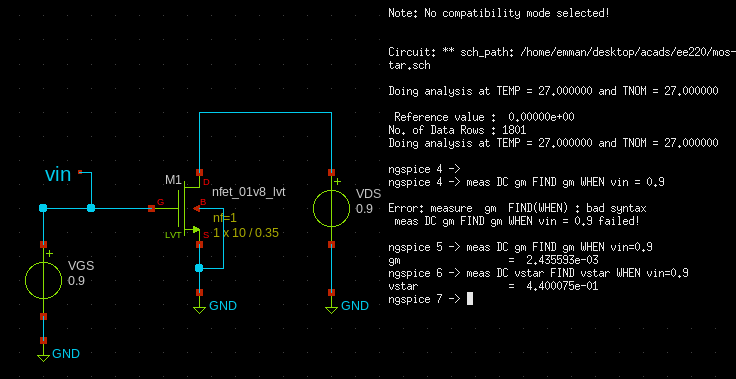
\includegraphics[scale=0.32]{gm-vstar.png}
	\label{fig:gm-vstar-NMOS} 
	\caption{$g_m$ and $v^*$}
\end{figure}
The values are obtained by using the MEAS command. Note that the TT corner is used.
\vspace{8pt}
\subsubsection{Simulations}
Flicker noise dominates the range $f < 500MHz$ whereas thermal noise dominates the region where $f > 500MHz$. With this, the flicker noise corner is at around $f=500MHz$. 
\begin{figure}[H]
	\centering
	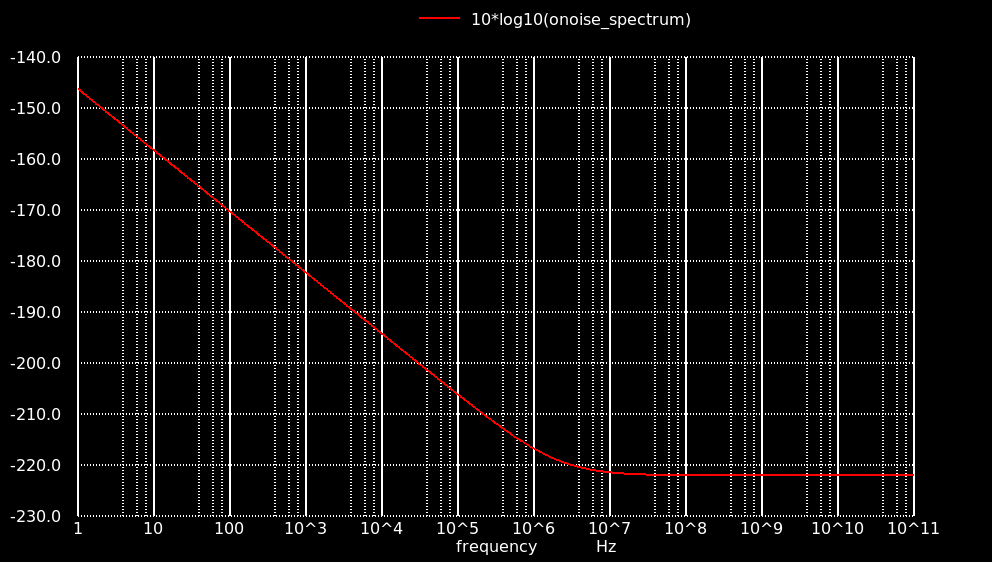
\includegraphics[scale=0.24]{noise-spectrum-35.png}
	\label{fig:noise-spectrum-35} 
	\caption{Output Noise PSD}
\end{figure}
\subsubsection{Estimating $\gamma$} Recall that in the absence of flicker noise, and assuming $\alpha=1$
\begin{equation*}
	\overline{i_{od}^{2}} = 4kT\gamma g_{m}
\end{equation*}
The total integrated noise power is equal to
\begin{align*}
	P_{i,noise} &= \int_{f1}^{f2}\overline{i_{od}^{2}}\;df \\
	&= \int_{f1}^{f2} 4kT\gamma g_{m}\; df \\
	&= 4kT\gamma g_m \cdot (f_2 - f_1)
\end{align*}
This means that if the integrated output noise power is obtained at the region where thermal noise is dominant, it is possible to directly compute for $\gamma$. To estimate, the total output noise power with 1-GHz bandwidth centered at around 90-GHz will be chosen. Since

\subsection{PMOS Noise}


\end{document}\textsl{}